\documentclass[12pt,twoside, a4paper, twocolumn]{article}
\usepackage[utf8]{inputenc}
\usepackage[brazil]{babel}
\usepackage[margin = 0.5in]{geometry}
\usepackage{amsmath}
\usepackage{amsthm}
\usepackage{amssymb}
\usepackage{amsthm}
\usepackage{setspace}
\usepackage[americanvoltages,fulldiodes,siunitx]{circuitikz}
\usepackage{lipsum}
\usepackage{pgfplots}
\usepackage{ifthen}
\usepackage{adjustbox}
\usepackage[section]{placeins}
\usepackage{hyperref}
\usepackage{graphicx}
\usepackage{adjustbox}
 
\pgfplotsset{compat=newest}
\graphicspath{ {./images/} }
\pgfplotsset{compat=newest}



%  #1 color - optional #2 x_0 #3 y_0 #4 x_f #5 y_f #6 name - optional  #7 true if adding lines to axis
 
\newcommand{\drawvector} [9] [color=cyan] {
   \draw[line width=1.5pt,#1,-stealth](axis cs: #2, #3)--(axis cs: #4, #5) node[anchor=south west]{$#6$};
 
  
 
\ifthenelse{\equal{#7}{true}}{
   \draw[line width=1pt,#1, dashed](axis cs: #4, #5)--(axis cs: #4, 0) node[anchor= north west]{$#8$};
   \draw[line width=1pt,#1, dashed](axis cs: #4, #5)--(axis cs: 0, #5) node[anchor=south east]{$#9$};
   }
   {}
}
 
\newcommand\deriv[2]{\frac{\mathrm d #1}{\mathrm d #2}}
 
 
\title{Segundo Relatório de Lab de Circuitos}
\author{Henrique da Silva \\ hpsilva@proton.me}
\date{\today}
\pgfplotsset{width = 10cm, compat = 1.9}
 
 
\begin{document}
\maketitle
\pagenumbering{gobble}
\newpage
%pagenumbering{roman}
\tableofcontents
\newpage



\section{Introdução}


\subparagraph*{Neste relatório, vamos discutir transistores, e como controlar a passagem de corrente alta por um circuito a partir de uma corrente mais baixa conectada em um transistor.}

\subparagraph*{Todos arquivos utilizados para criar este relatório, é o relatorio em si estão em:  \url{https://github.com/Shapis/ufpe_ee/tree/main/4th semester/lab circuitos}}




\section{O Transistor}
\subparagraph*{}
\begin{center}
    \begin{circuitikz}
        \draw
        (0,0) to[battery1,  invert] (0,2) -- (0,2) -- (1,2)
        ;
        \draw (0,-0.05)
        node[rground]{};
        \draw (1.85,2.77) node [npn,anchor=C] (npn) {}
        (npn.collector);
        \draw (1.85,1.21) -- (1.85,0) -- (0,0);
        \draw (1.85,0) -- (4,0) to[battery1, invert] (4,4) to[R] (1.85,4) to[rmeter, t=L] (1.85,2.5);
        % \draw (2,2)
        % node[ocirc,  label=2:$V_{a}$]{};
        % \draw (4,2)
        % node[ocirc,  label=2:$V_{b}$]{};
    \end{circuitikz}
\end{center}

\subparagraph*{Neste caso o transistor impediria passagem de corrente no circuito maior até haver uma tensão mínima de aproximadamente $0.7V$ no circuito menor}

\subparagraph*{Podemos também olhar pra ele da seguinte maneira:}



\begin{center}
    \begin{circuitikz}
        \draw (2,2)
        node[ocirc,  label=0:$I_E$]{}
        ;
        \draw (0 ,-1)
        node[ocirc,  label=270:$I_B$]{}
        ;
        \draw (4 ,-1)
        node[ocirc,  label=270:$I_C$]{}
        ;

        \draw (2,2) -- (2,1) -- (3,1) to[cI, l=$\beta I_B$] (3,-1) -- (4,-1);
        \draw (2,1) -- (1,1) to[battery1, a=$0.7V$] (1,-1) -- (0,-1);
    \end{circuitikz}
\end{center}

\subparagraph*{Que nos dá uma situação em que se o potencial em $I_E$ for maior que o potencial em $I_B$  nós ativamos a fonte de corrente com $\beta I_B$}

\subparagraph*{Podemos ver então $\beta$ como a proporção entre a corrente no circuito principal e a corrente no circuito de ativação.}



\begin{equation}
    \begin{aligned}
        I_E = I_B + \beta I_B \\
    \end{aligned}
\end{equation}

\section{Analise teorica}

\subsection{Obtendo a resistencia de Thevenin/Norton}


\subparagraph*{Primeiro vale lembrar que a resistência de Thevenin e a de Norton são iguais. Logo obtendo uma também obteremos a outra.
}

\subparagraph*{Neste caso, resolvendo o sistema vamos obter que esta resistência é igual a $R_{c}$}

\begin{equation}
    \begin{aligned}
        R_c = R_{th} = R_{no}
    \end{aligned}
\end{equation}

\subsection{Obtendo a tensão de Thevenin e a corrente de Norton}

\subparagraph*{Basta obtermos um deles, pois temos a seguinte relação:}

\begin{equation}
    \begin{aligned}
        V_{th} = I_{no} * R_{th/no}
    \end{aligned}
\end{equation}

\subparagraph*{E vou usar a convenção que a soma de todas correntes de saem de um nó é = a 0 para simplificar os cálculos e minimizar erros de sinal}

\subparagraph*{Isto me dá as seguintes equações:}

\begin{equation}
    \begin{aligned}
        \frac{V_b - V_{cc}}{R_1} + \frac{V_b}{R_2} - I_b & = 0 \\
        \frac{V_e - V_{cc}}{R_e} + I_b + \beta*I_b       & = 0 \\
        -\beta*I_b + \frac{V_c}{R_c}                     & = 0 \\
        V_b + {V_be0} - V_e                              & = 0 \\
    \end{aligned}
\end{equation}

\section{Resultados Preliminares}

\subparagraph*{As simplificações e resoluções das equações (4) foram feitas em python e estão dentro do zip enviado e na pasta do github mencionada na introdução}

\subparagraph*{As resoluções foram analisando o caso particular em que $V_{cc} = 10V$, $R_1 = 220 \varOmega$, $R_2 = 1500 \varOmega$, $R_e = 150\varOmega$, $R_c = 1500\varOmega$, $\beta = 100$, $V_{be0} = 0.7V$}

\subparagraph*{Observação: Na aula foi feito $R_1 = 200 \varOmega$, e no roteiro o $R_1 = 220 \varOmega$ entao resultados obtidos são um pouco diferentes dos resultados de aula, porém testando com $R_1 = 200 \varOmega$ obtenho exatamente os mesmos valores obtidos em aula.}


\subparagraph*{Resultados para potência de Thevenin maxima}

\begin{center}
    \begin{tabular}{ |ccc| }
        \hline
        $V_{th}$     & $\rightarrow$ & $5.66V$          \\
        $R_{th}$     & $\rightarrow$ & $1500 \varOmega$ \\
        $I_{no}$     & $\rightarrow$ & $0.00377 A$      \\
        $R_{no}$     & $\rightarrow$ & $1500 \varOmega$ \\
        $G_{no}$     & $\rightarrow$ & $0.00067 S$      \\
        $R_{max}$    & $\rightarrow$ & $1500 \varOmega$ \\
        $P_{max}$    & $\rightarrow$ & $0.00534W$       \\
        $P_{V_{cc}}$ & $\rightarrow$ & $0.1W$           \\

        \hline
    \end{tabular}
\end{center}

\section{Resultados experimentais}

\paragraph*{Com o circuito montado notei uma discrepância entre as tensões de Thevenin, e das tensões em RL esperadas e das encontradas.}

\paragraph*{Isto ocorreu devido a inicialmente ter calculado o \emph{ganho} $\beta$ do transistor como $100$, é o valor real, refazendo a análise teórica para bater com os resultados encontrados está mais próximo de $260$.}

\paragraph*{Além disso a tensão $V_{be0}$ encontrada experimentalmente foi de $0.68V$, e não $0.7V$ como já havíamos utilizado na análise teórica anteriormente.}

\paragraph*{Com isto em mente podemos interpretar a \emph{tabela de dados experimentais} que será apresentada abaixo:}

\subsection{Tabela de dados}

\begin{center}
    \begin{tabular}{ |ccc| }
        \hline
        $V_{th}$ & $\rightarrow$ & $6V$ \\
        \hline
    \end{tabular}
\end{center}

\begin{center}
    \begin{tabular}{ |c|c|c| }
        \hline
        $R_L$            & $V_{RL}$ & $Potencia$ \\
        $92\varOmega$    & $0.38$   & $0.00157W$ \\
        $980\varOmega$   & $2.41$   & $0.00592W$ \\
        $2200\varOmega$  & $3.59$   & $0.00586W$ \\
        $22150\varOmega$ & $5.6$    & $0.00142W$ \\
        \hline
    \end{tabular}
\end{center}

\subparagraph*{Pela dedução teórica, a potência máxima deveria ocorrer quando $R_L = R_{c}$, que no caso eh $R_{L} = 1500 \varOmega$, e esta potência deveria ser $0.00587W$.}

\subparagraph*{O resultado está próximo, apesar de não termos testado $R_{L} = 1500\varOmega$, as potencias entre $1000\varOmega$ e $2000\varOmega$ são muito próximas, e estão também muito próximas a potência máxima teórica. }

\subparagraph*{Que de fato, é o comportamento esperado.}

\subsection{Convergencia para o limite de $R_L \rightarrow \infty\varOmega$}

\subparagraph*{Também podemos observar que a tensão sobre $R_L$ converge para $V_{th}$ conforme $R_L$ cresce. E isto é dado por:}

\begin{equation}
    V_{L} = V_{th} * \frac{R_{L}}{R_{L} + R_{th}}
\end{equation}

\subparagraph*{Substituindo os valores encontrado acima também verificamos que nossos resultados são coerentes, como por exemplo para o $R_L = 22150\varOmega$:}

\begin{equation}
    V_{L} = 6 * \frac{22150}{23650} = 5.6V
\end{equation}

\section{Grafico teoricos}

\subparagraph*{Por esta analise obtivemos $V_{th} = 5.84V$, $R_{th} = 1346.2\varOmega$}
\subparagraph*{Que estao bem proximos dos valores encontrados experimentalmente, $V_{th} = 6V$ e $R_{th} = 1500\varOmega$}
\paragraph*{}
\begin{adjustbox}{scale=0.60}
    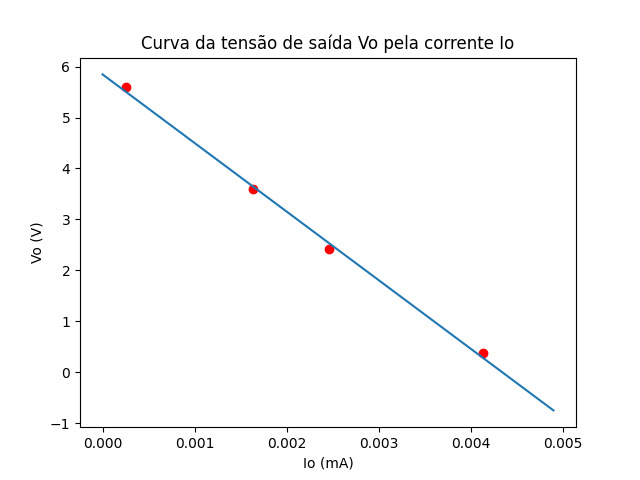
\includegraphics{Figure_1.png}
\end{adjustbox}

\section{Conclusoes}

\subparagraph*{Vimos que podemos um controlador de corrente, utilizando um transistor e um sistema de corrente mais baixa.}

\subparagraph*{Este circuito tem propriedades bastante convenientes, como por exemplo a sua resistência de Thevenin se resume a ser igual a resistência $R_c$.}

\subparagraph*{E podemos limitar a corrente de saída do circuito, utilizando um resistor $R_L$ de valor adequado.}

\end{document}

